
\begin{titlepage}
\begin{tikzpicture}[remember picture,overlay]
\coordinate (A) at (0,0);

\node[at=(current page.center),
      opacity=0.1,
      fill=white,
      inner sep=0pt,
     ]  {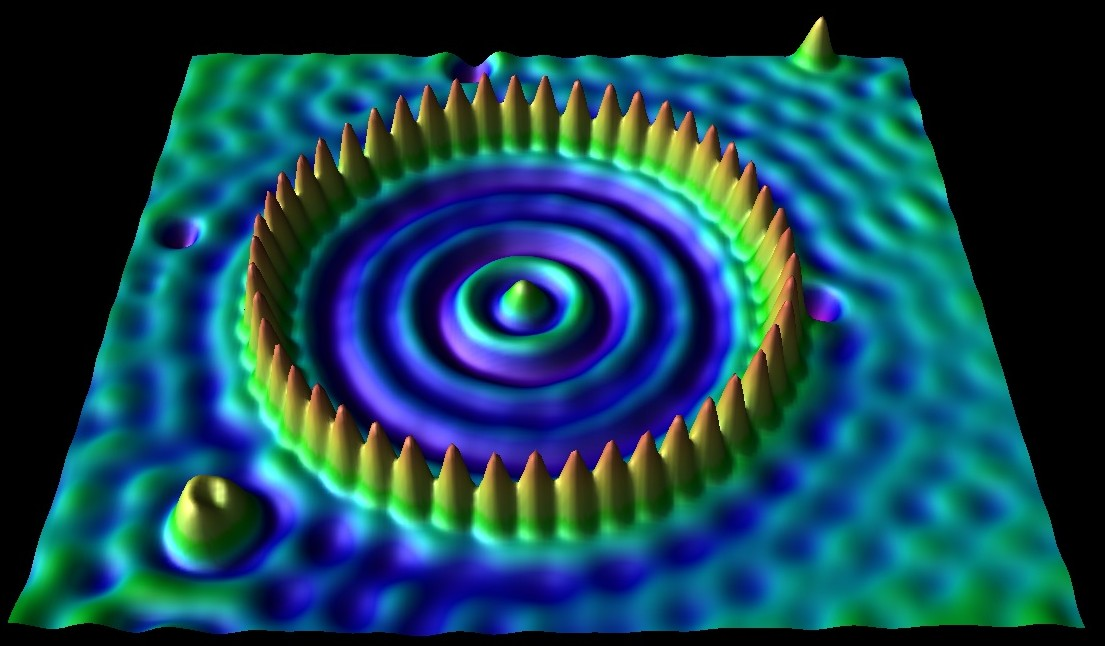
\includegraphics[width=\paperwidth,height=\paperheight]{./Figures/Beamer/qc2}};
     

\node[anchor=north east,
scale=0.07,
inner sep=0pt,
opacity=1,
](iicologo) 
at (current page.north east) {
\includegraphics{./Figures/Beamer/LOGO_IICO_AZUL.png}};

\node[anchor=north west,
scale=0.15,
inner sep=0pt,
opacity=1,
](iicologo) 
at (current page.north west) {
\includegraphics{./Figures/Beamer/LOGO_UASLP_AZUL.png}};      
     
     
\node[font=\fontsize{7}{14}\selectfont, 
      text width=30cm,
      anchor=north,
	  inner sep=0pt,
	  yshift=-0.5cm,
      blue,
      align=center] (uni) at (current page.north) { 
   UNIVERSIDAD AUTONOMA DE SAN LUIS POTOSI\\
   FACULTAD DE CIENCIAS\\
   POSGRADO EN CIENCIAS APLICADAS        
       };     
     
%\node[font=\fontsize{14}{10}\selectfont, 
%      text width=17cm,
%      anchor=center,
%      inner sep=0pt,
%      yshift=1.8cm,
%      color=blue!20!black!80,
%      align=center] (title) at (current page.center) { 
%      
%           };
%       
\node[%
%font=\bfseries\fontsize{20}{10}\selectfont, 
text width=4cm,
anchor=center,
inner sep=0pt,
yshift=1cm,
color=blue!20!black!80,
align=center,
scale=3] (title) at (current page.center)  { 
	Anisotropias 'Opticas  de pozos cu\'anticos acoplados  asim\'etricos de GaAs(001)
};
       
\node[below = of title,
font=\fontsize{8}{14}\selectfont, 
text width=30cm,
inner sep=0pt,
yshift=1cm,
align=center] (author) {
                        OSCAR RUIZ CIGARRILLO\\
                         };       
       
\node[below = of author,
font=\fontsize{8}{14}\selectfont, 
text width=30cm,
inner sep=0pt,
yshift=0,
align=center] (profesor) { 
		                {\color{blue}Asesores de tesis} \\
                        Dr. Luis Felipe Lastras Martinez\\
                        Dr. Edgar Armando Cerda Mendez
                     };   
\node[below = of profesor,
font=\fontsize{5}{14}\selectfont, 
text width=30cm,
inner sep=0pt,
yshift=0.5cm,
align=center] (date) {SAN LUIS POTOSÍ, MÉXICO, \today};                     
                             
\end{tikzpicture}

\
\end{titlepage}